\section{Auswertung}
\subsection{Rohrresonator}
Zunächst wird das Frequenzspektrum von einem bis zwölf aneinander gereihten Zylindern der jeweiligen Länge $50$mm
in einem Frequenzbereich von $0,1$kHz bis $12$kHz mit einem 2-Kanal-Oszilloskop aufgenommen.
Diese Messung wird mit der Software des Computers wiederholt.
Exemplarisch werden im folgenden die beiden Messungen mit einem, fünf und zwölf Zylindern dargestellt.
Es wird deutlich, dass beide Frequenzspektren ähnlich aussehen. Allerdings ist die Auflösung 
des Spektrums, welches von der Computersoftware aufgezeichnet wurde höher. Es ist daher sinnvoll im Folgenden
diese zu verwenden.

\begin{figure}[H]

    \centering
    \subfloat[Das Frequenzspektrum eines einzelnen Rohrresonators der Länge $50$mm (Computersoftware).]{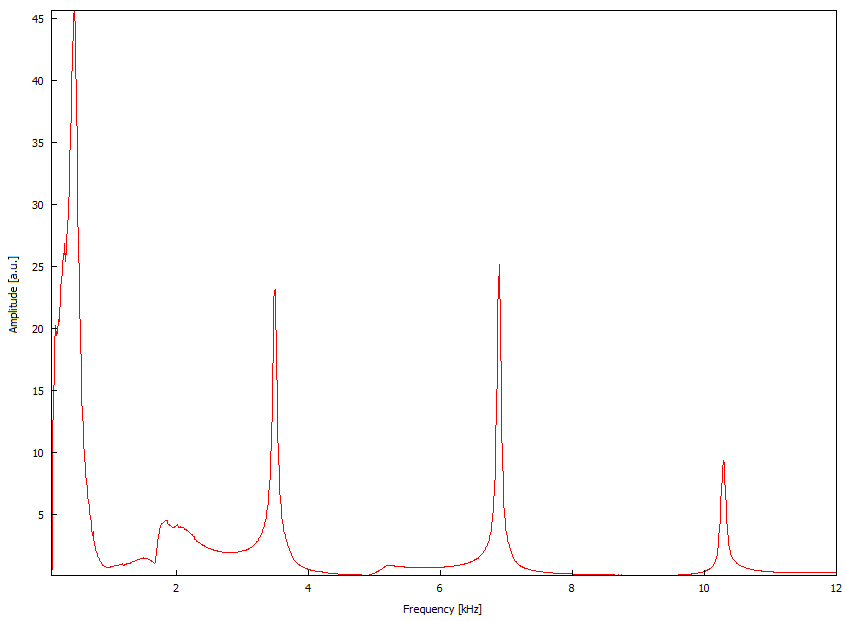
\includegraphics[width=0.45\textwidth]{data/Vorbereitung/Spektrum_1.png}}\hfil
    \subfloat[Das Frequenzspektrum eines einzelnen Rohrrensonators der Länge $50$mm (per Oszilloskop).]{\includegraphics[width=0.45\textwidth]{example-image-b}}\hfil 
    
    \subfloat[Das Frequenzspektrum von fünf Rohrresonatoren der jeweiligen Länge $50$mm (Computersoftware).]{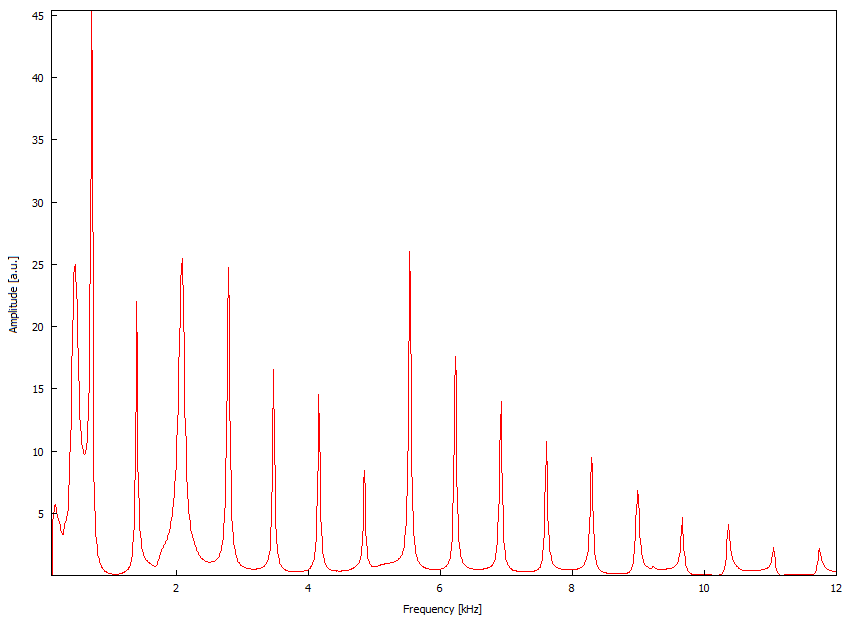
\includegraphics[width=0.45\textwidth]{data/Vorbereitung/Spektrum_5.png}}\hfil
    \subfloat[Das Frequenzspektrum von fünf Rohrrensonatoren der jeweiligen Länge $50$mm (per Oszilloskop).]{\includegraphics[width=0.45\textwidth]{example-image-b}}\hfil

    \subfloat[Das Frequenzspektrum von zwölf Rohrresonatoren der jeweiligen Länge $50$mm (Computersoftware).]{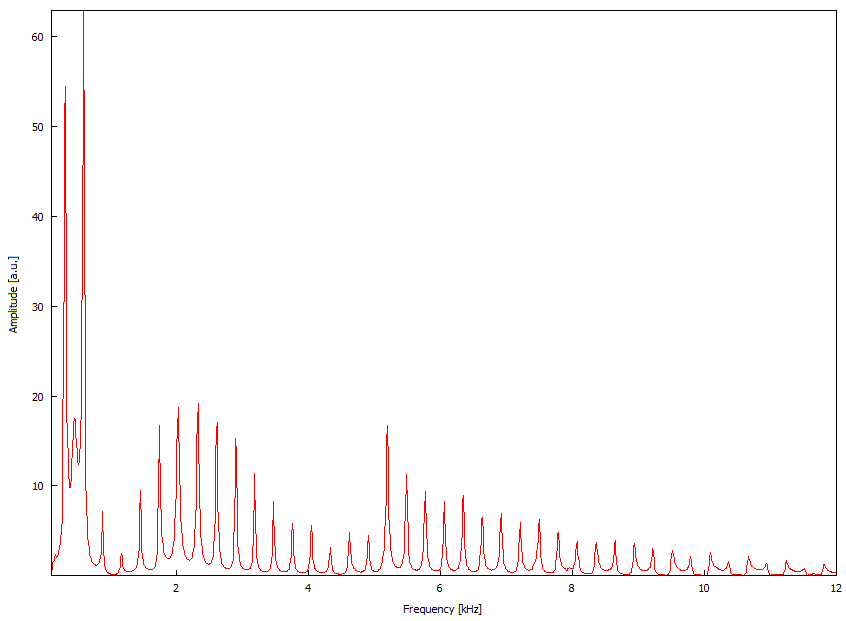
\includegraphics[width=0.45\textwidth]{data/Vorbereitung/Spektrum_12.png}}\hfil
    \subfloat[Das Frequenzspektrum von zwölf Rohrrensonatoren der jeweiligen Länge $50$mm (per Oszilloskop).]{\includegraphics[width=0.45\textwidth]{example-image-b}}
    \caption{}\label{figure}
\end{figure}

\subsection{Wasserstoffatom}
Nun wird der Kugelresonator (Wasserstoffatom) betrachtet. Hierbei wird ein Frequenzspektrum
von $0,1$kHz bis $12$kHz in $5$Hz-Schritten aufgenommen. Der Winkel zwischen Mikrofon und Lautsprecher betraägt $180°$.
Die gefunden Resonanzfrequenzen werden anschließend erneut händisch mit dem Sinusgenerator über das Oszilloskop vermessen.
Dies beinhaltet die Ordnung der Resonanz, die Amplitude sowie die Phasenverschiebung neben der Resonanzfrequenz.
Für die Resonanzfrequenzen $X$kHz, $Y$kHz, $Z$kHz und $W$kHz wird die Winkelabhängigkeit im Bereich $0°$ bis $180°$ in $10°$-Schritten betrachtet.\\
Zur Analyse der Aufspaltung wird ein Frequenzspektrum in $1$Hz-Schritten im Bereich $1,8$ und $2,8$kHz mit eingesetzten
verschiedener Blenden aufgenommen. Die Abhängigkeit der Resonanzfrequenz vom Winkel wird bei eingesetzter $9$mm Blende 
im Winkelbereich $0°$ bis $180°$ betrachtet.

\subsubsection*{Resonanzfrequenz}
Im Frequenzbereich zwischen $0,1$ und $12$kHz ergibt sich bei einem Winkel von $180°$ das in Abbildung \ref{fig:kugel_res}
dargestellte Frequenzspektrum

\begin{figure}
    \center
    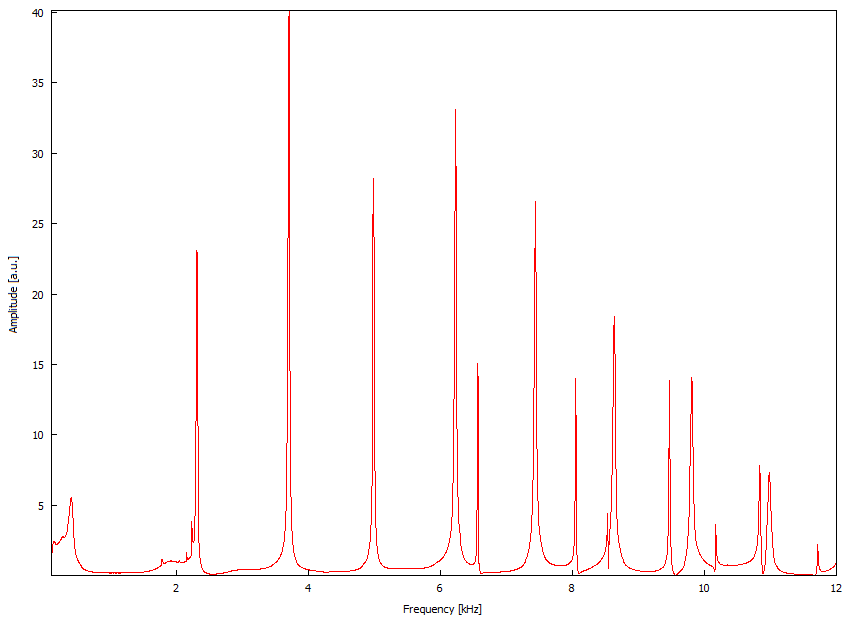
\includegraphics[width=0.7\textwidth]{data/Wasserstoffatom/Ohne_Ring/Spektrum_180_first.png}%{bilder/plots/kugel_180_plot.pdf}
    \caption{Das Hochauflösende Spektrum des Kugelresonators (Wasserstoffatommodells), bei einem 
    festen Polarwinkel von $180°$. Dabei ist die Frequenz in kHz gegen die Amplitude in willkürlichen Einheiten aufgetragen.}
    \label{fig:kugel_res}
\end{figure}

Die genauere Betrachtung der Resonanzfrequenzen $\nu_{res}$ aus Abbildung \ref{fig:kugel_res} mithilfe des Oszilloskops
liefert die jeweilige Ordnung, Amplitude und Phasenverschiebung.

\begin{table}[H]
    \center
    \caption{Die zu den Resonanzfrequenten $\nu_{Res}$ gehörigen Ordnungen, Amplituden und Phasenverschiebungen.}
    \begin{tabular}{l l l c}
        \toprule
        Ordnung & $\nu_{Res}\,/\,$kHz & Amplitude$\,/\,$V & $\varphi\,/\,°$\\
        \midrule
        1 &0,4 &4,3 &-102 \\
        2 &2,301 &76 &70 \\
        3 &3,694 &231 &-78 \\
        4 &4,979 &187 &90 \\
        5 &6,221 &249 &-30 \\
        6 &7,433 &239 &170 \\
        7 &8,042 &143 &-14 \\
        8 &8,630 &189 &20 \\
        9 &9,465 &155 &-150 \\
        10 &9,807 &159 &-133 \\
        \bottomrule
    \end{tabular}
\end{table}

\subsubsection{Die Winkelabhängigkeit der Resonanzfrequenzen}
Nun wird die Druckamplitude der Resonanzfrequenzen $2,301\,$kHz, $3,694\,$kHz, $4,979\,$kHz und $7,433\,$kHz 
in Abhängigkeit des Winkels $\theta$ betrachtet.\\
Deutlich zu ernennen sind die Keulen in $180°$-Richtung, sowie eine schwache Ausprägung in $90°$-Richtung.

\begin{figure}[H]
    \centering
    \subfloat[Die Druckamplitude bei der Resonanzstelle $X$kHz im Vergleich zu einem $2{p}_0$.]{\includegraphics[width=0.45\textwidth]{example-image-a}}\hfil
    \subfloat[Die Druckamplitude bei der Resonanzstelle $Y$kHz im Vergleich zu einem $3{d}_0$-Orbital.]{\includegraphics[width=0.45\textwidth]{example-image-a}}\hfil 
    
    \subfloat[Die Druckamplitude bei der Resonanzstelle $Z$kHz im Vergleich zu einem $4{f}_0$-Orbital.]{\includegraphics[width=0.45\textwidth]{example-image-a}}\hfil
    \subfloat[Die Druckamplitude bei der Resonanzstelle $W$kHz im Vergleich zu einem $6{h}_0$-Orbital.]{\includegraphics[width=0.45\textwidth]{example-image-a}}\hfil 
    \caption{}\label{figure}
\end{figure}
\subsubsection*{Aufspaltung der Zustände}
Nun werden verschiedene Zwischenringe zwischen den beiden Halbkugel eingesetzt. Exemplarische wird im folgenden das Zwischenstück
mit einer Ringbreite von $3$mm betrachtet. In Abbildung \ref{fig:aufspaltung} sind die zwei resultierenden Resonanzfrequenzen
deutlich. Die Drehimpulsquantenzahl $l$ muss daher gleich eins sein und bestätigt die Annahme, dass es sich um ein 2p$_0$-orbital handelt.  

\begin{figure}[H]
    \center
    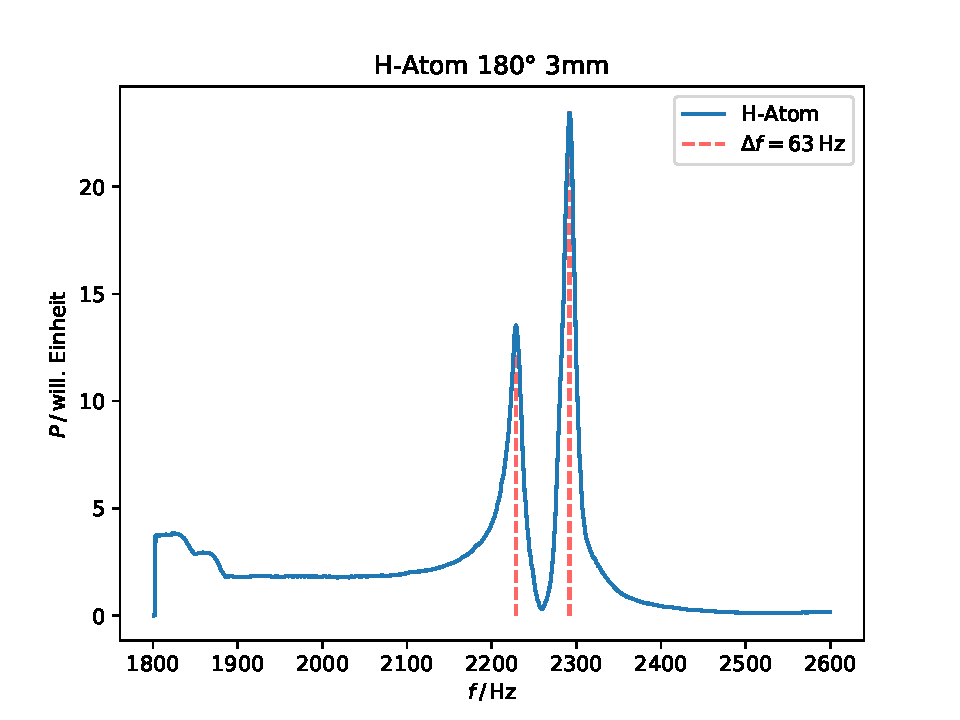
\includegraphics[width=0.8\textwidth]{plots/Hatom/zustandsaufspaltung.pdf}
    \caption{Aufspaltung der Resonanz bei $2,301$kHz in zwei Resonanzfrequenzen.}
    \label{fig:aufspaltung}
\end{figure}

Trägt man nun die die Resonanzfrequenz-Differenz $\Delta\nu$ gegen die Zwischenringbreite auf,
so wird deutlich, dass sich dies annähernd linear verhält. Analogon hierfür wäre die Aufspaltung der Zustände eines
Wasserstoffatoms in einem extern anliegendem Magnetfeld (Zeeman-Effekt).

\begin{figure}[H]
    \center
    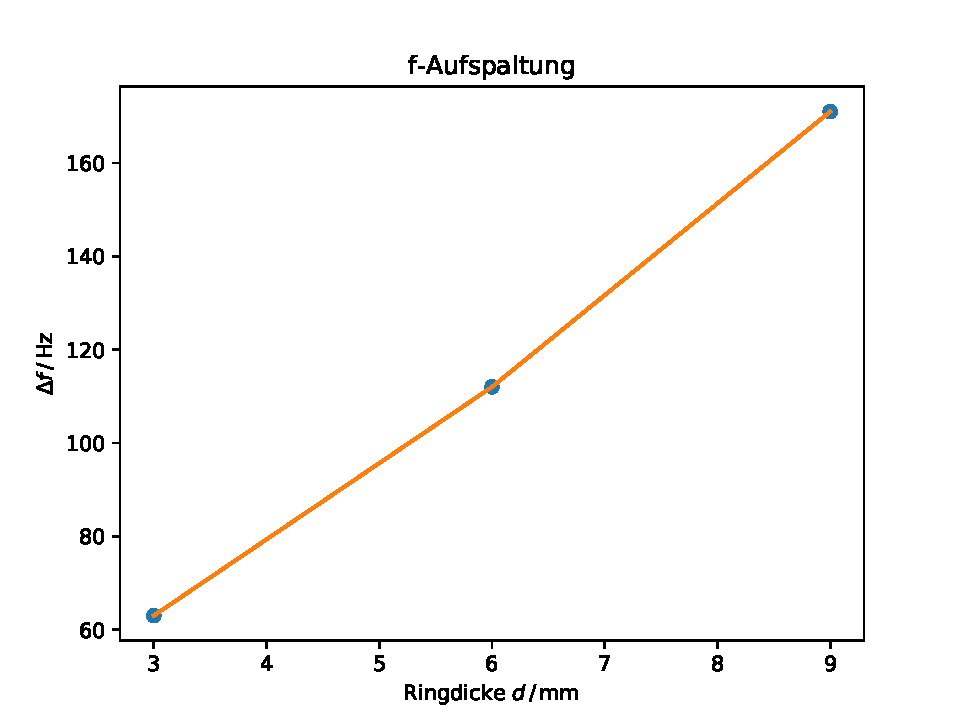
\includegraphics[width=0.8\textwidth]{plots/Hatom/faufspaltung.pdf}
    \caption{Abhängigkeit zwischen der Resonanzfrequenz-Differenz $\Delta\nu$ und der Ringbreite.}
    \label{fig:d_res}
\end{figure}

\subsubsection*{Zustandsaufspaltung und deren Winkelabhängigkeit}
Für einen Zwischenring der Ringbreite $9$mm wird im Folgenden die Wineklabhängigkeit betrachtet (Abbildung \ref{fig:9mm_winkel}).

\begin{figure}[H]
    \center
    \includegraphics[width=0.5\textwidth]{example-image-a}
    \caption{Druckamplitude gegen den Winke $\theta$ aufgetragen.}
    \label{fig:9mm_winkel}
\end{figure}

Für die Aufspaltung bei $180°$ ergibt sich das Frequenzspektrum aus Abbildung \ref{fig:9mm_res}.
Die Resonanzfrequenz $X$kHz entspricht $m=0$ und $l=1$. Für die Resonanzfrequenz $Y$kHz folgt $m=\pm 1$ und $l=1$.
\begin{figure}[H]
    \center
    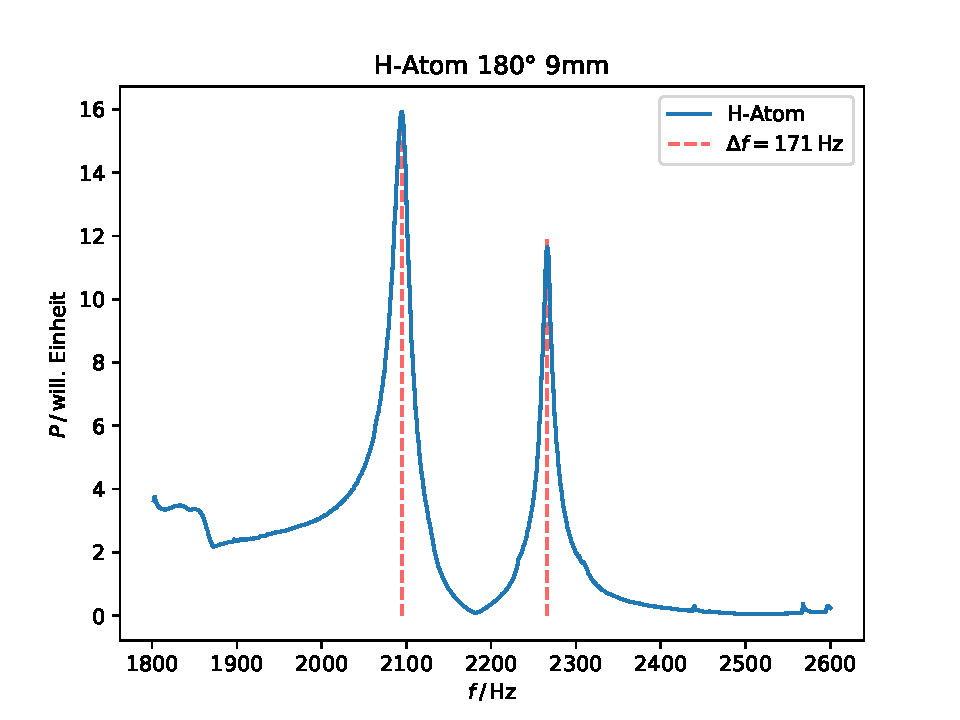
\includegraphics[width=0.7\textwidth]{plots/Hatom/zustandsaufspaltung_9.pdf}
    \caption{Die Aufspaltung der Resonanz bei Verwendung eines Zwischenrings der Breite $9$mm bei einem Winkel $\theta$ von $180°$.}
    \label{fig:9mm_winkel}
\end{figure}
\newpage
\subsection{Wasserstoffmolekül}
\subsubsection*{Einfluss des Blendendurchmessers auf die Resonanzfrequenz}
Nun werden zwei Kugelresonatoren über eine Blende, welche die Kopplungsstärke wiederspiegelt, gekoppelt.
Zur Untersuchung wird zunächst ein Frequenzspektrum im Bereich von $2,2$kHz bis $2,5$kHz in $1$Hz-Schritten bei verschiedenen
Blenden von $10$mm, $16$mm, $20$mm betrachtet.\\

Für das Resonanzfrequenz $\nu$ in Abhängigkeit des Blendendurchmessers zeigt sich folgender in Abbildung \ref{fig:blende_mol}
Verlauf.
\begin{figure}[H]
    \center
    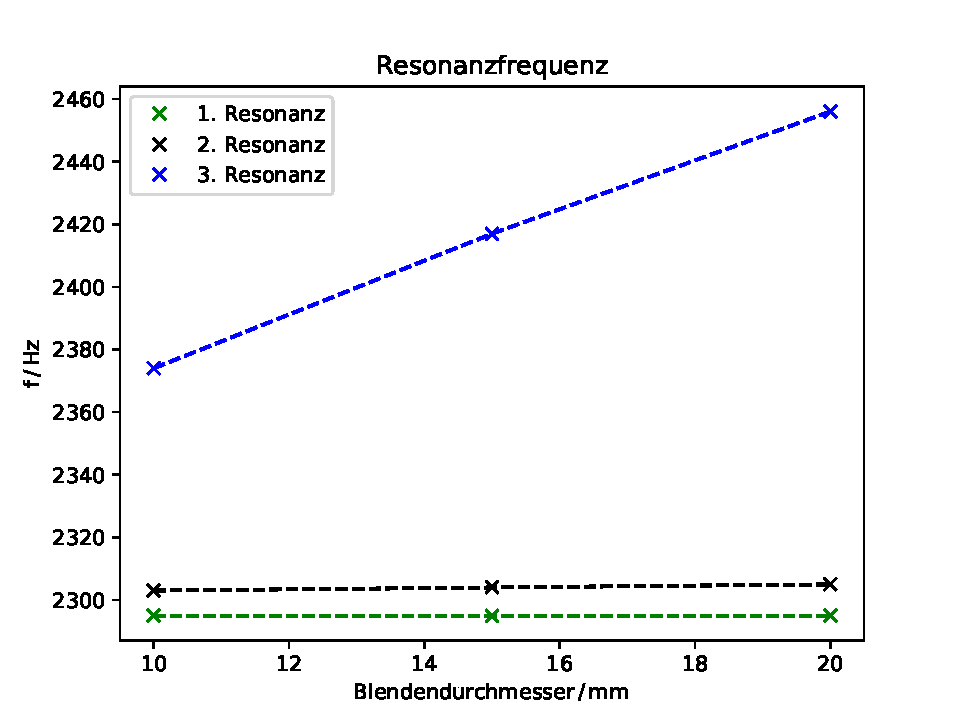
\includegraphics[width=0.7\textwidth]{plots/Hatom/res_blende.pdf}
    \caption{Abhängigkeit der 3 Resonanzfrequenzen zum Blendendurchmesser.}
    \label{fig:blende_mol}
\end{figure}

\subsubsection*{Winkelabhängigkeit der Resonanzfrequenz}
Für den Blendendurchmesser von $15$mm zeigen sich die drei Resonanzen, dargestellt in Abbildung \ref{fig:blende_16_res},
bei den Frequenzen $\nu$ von $2,297$kHz, $2,304$kHz und $2,416$kHz.
\begin{figure}[H]
    \center
    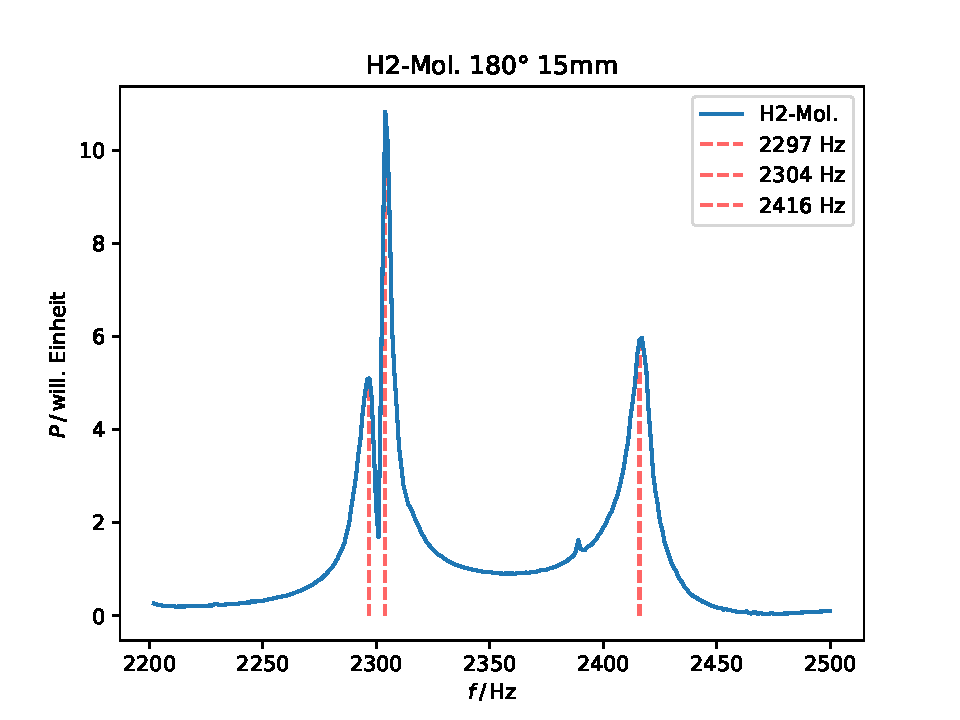
\includegraphics[width=0.7\textwidth]{plots/Hatom/zustandsaufspaltung_mol15.pdf}
    \caption{Frequenzspektrum bei einem Winkel $\theta=180°$. Zu sehen sind die Resonanzenfrequenzen $\nu$ bei $2,297$kHz, $2,304$kHz und $2,416$kHz.}
    \label{fig:blende_16_res}
\end{figure}

Im Folgenden werden für diese vier Resonanzfrequenzen die Druckamplituden in Abhängigkeit des Winkels $\theta$ betrachtet und die Phasenverschiebung in Tabelle \ref{tab:mol_diff} aufgelistet.
Daraus lassen sich die Symmetrien der Zustände definieren. Für eine Phasendifferenz von $0°$ spricht man von einem symmetrischen und bei einer Phase von $180°$ von einem antisymmetrischen Zustand.
%VERGLEICHE LASSE
\begin{figure}[H]
    \centering
    \subfloat[Die Druckamplitude bei der Resonanzstelle $2,297$kHz im Vergleich zu einem $2{p}_0$.]{\includegraphics[width=0.45\textwidth]{example-image-a}}\hfil
    \subfloat[Die Druckamplitude bei der Resonanzstelle $2,304$kHz im Vergleich zu einem $3{d}_0$-Orbital.]{\includegraphics[width=0.45\textwidth]{example-image-a}}\hfil 
    
    \subfloat[Die Druckamplitude bei der Resonanzstelle $2,416$kHz im Vergleich zu einem $4{f}_0$-Orbital.]{\includegraphics[width=0.45\textwidth]{example-image-a}}\hfil
    \caption{}
    \label{fig:polarplots}
\end{figure}
Somit folgt für die Zustände !!!!!!!!!!

\begin{table}
    \center
    \caption{}
    \begin{tabular}{c| c c c c}
        \toprule
        Ordnung & $\nu_{Res}\,/\,$kHz & obere Phasendiff. $\,/\,°$ & untere Phasendiff. $\,/\,°$ & $\Delta$ Phasendiff. $\,/\,°$\\
        \midrule
        1 &2,296 &-135 &10 &145 \\
        2 &2,303 &-126 &30 &156 \\
        3 &2,418 &53 &-128 &181 \\
        \bottomrule
    \end{tabular}
    \label{tab:mol_diff}
\end{table}

\subsection{1-dim-Festkörper}
\subsubsection*{Resonatorkette}
Nun wird ein Frequenzspektrum einer Resonatorkette betrachtet die mit jeweils $16$mm-Blenden versehen werden.
In Abbildung \ref{fig:reskette_res} prägen sich vier Bereiche aus, die mit Maxima gefüllt sind. DAbei entspricht dies der Anzahl der Maxima der verwendeten Zylinder.
Überträgt man dies auf das Analogon des 1-dim-Festkörpers so lässt sich sagen, dass durch jeden Zylinder ein Band hinzugeführt wird, auf dem die Elektronen
in eine Festkörper Zustaände einnehmen können. Die leeren Bereiche sind dabei bandlücken und beschreiben somit die 'verbotenden' Zonen im Festkörper in denen keine Elektronenzustände vorliegen.


\begin{figure}[H]
    \centering
    \subfloat[Frequenzspektrum für eine Resonatorkette aus zwei Resonatorgliedern (Rohrzylindern) mit einer jeweiligen Länge von $50$mm und einer $16$mm-Blende als Zwischenstück.]{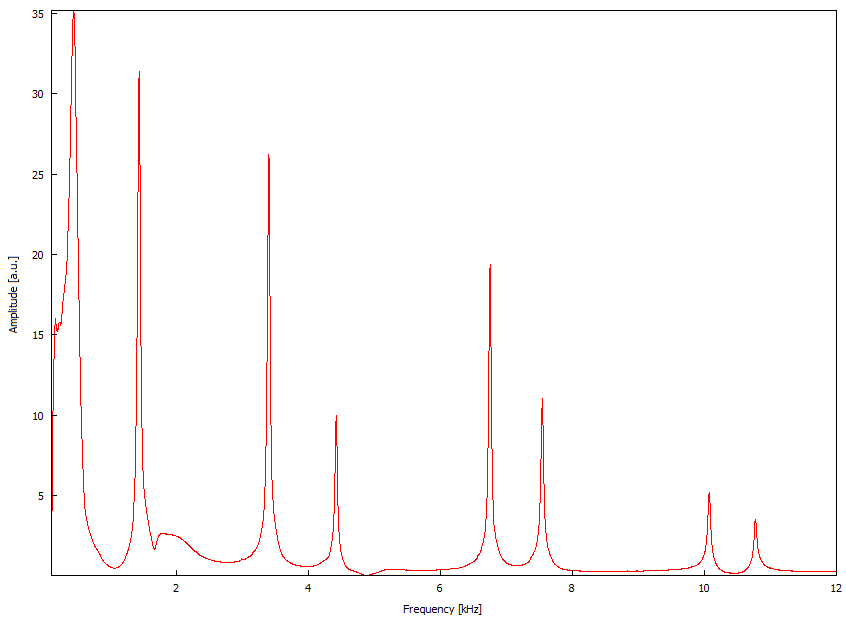
\includegraphics[width=0.45\textwidth]{data/Festkoerper/16mm/Spektrum_2.png}}\hfil
    \subfloat[Frequenzspektrum für eine Resonatorkette aus vier Resonatorgliedern (Rohrzylindern) mit einer jeweiligen Länge von $50$mm und einer $16$mm-Blende als Zwischenstück.]{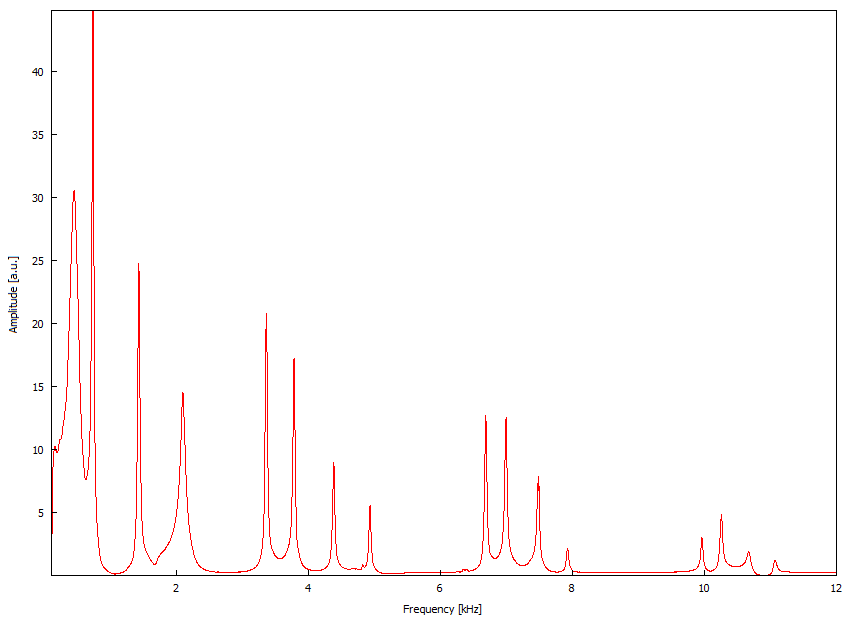
\includegraphics[width=0.45\textwidth]{data/Festkoerper/16mm/Spektrum_4.png}}\hfil 
    
    \subfloat[Frequenzspektrum für eine Resonatorkette aus zehn Resonatorgliedern (Rohrzylindern) mit einer jeweiligen Länge von $50$mm und einer $16$mm-Blende als Zwischenstück..]{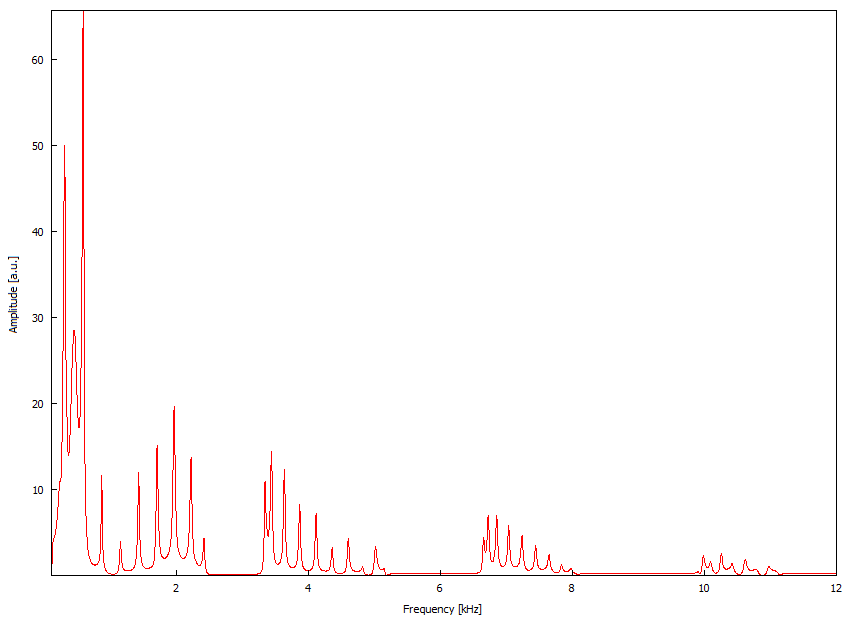
\includegraphics[width=0.45\textwidth]{data/Festkoerper/16mm/Spektrum_10.png}}\hfil
    \caption{}
    \label{fig:reskette_res}
\end{figure}

\subsubsection{Resonatorkette mit verschiedenen Blendendurchmessern}
Die Größe des Blendendurchmessers spiegelt im Analogon des 1-dim-Festkörpers ein unterschiedlich starkes
Potenzial wieder, sodass die Elektronen unterschiedlich stark lokalisiert auf ihren Bändern sind.
Dies wird deutlich, wenn man sich das Frequenzspektrum zweier Resonatorketten mit unterschiedlichen Blenden betrachtet.
Dazu ist in Abbildung \ref{fig:fest_2_blende} jeweils das Frequenzspektrum einer Resonatorkette mit zwei Zylindern und einer $10$mm-Blende
und gleiche Resonatorkette mit einer $13$mm-Blende dargestellt.\\
\begin{figure}[H]
    \centering
    \subfloat[Frequenzspektrum einer Resonatorkette bestehend aus zwei Rohrzylindern der Länge 50mm und eine Blende mit dem Durchmesser von 10mm.]{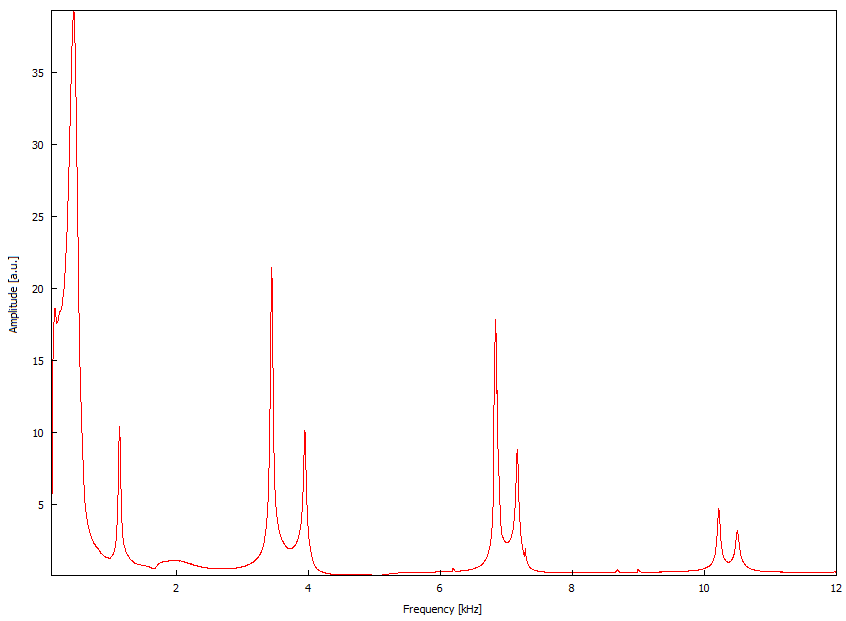
\includegraphics[width=0.45\textwidth]{data/Festkoerper/10mm/Spektrum_2.png}}\hfil
    \subfloat[Frequenzspektrum einer Resonatorkette bestehend aus zwei Rohrzylindern der Länge 50mm und eine Blende mit dem Durchmesser von 13mm.]{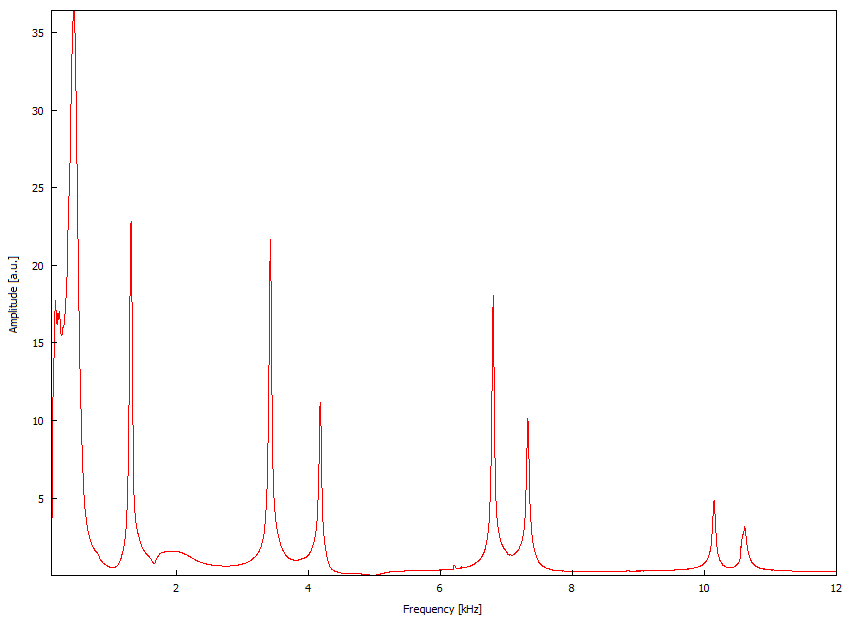
\includegraphics[width=0.45\textwidth]{data/Festkoerper/13mm/Spektrum_2.png}}\hfil 
    \caption{}
    \label{fig:fest_2_blende}
\end{figure}

\begin{figure}[H]
    \centering
    \subfloat[Frequenzspektrum einer Resonatorkette bestehend aus vier Rohrzylindern der Länge 50mm und eine Blende mit dem Durchmesser von 10mm.]{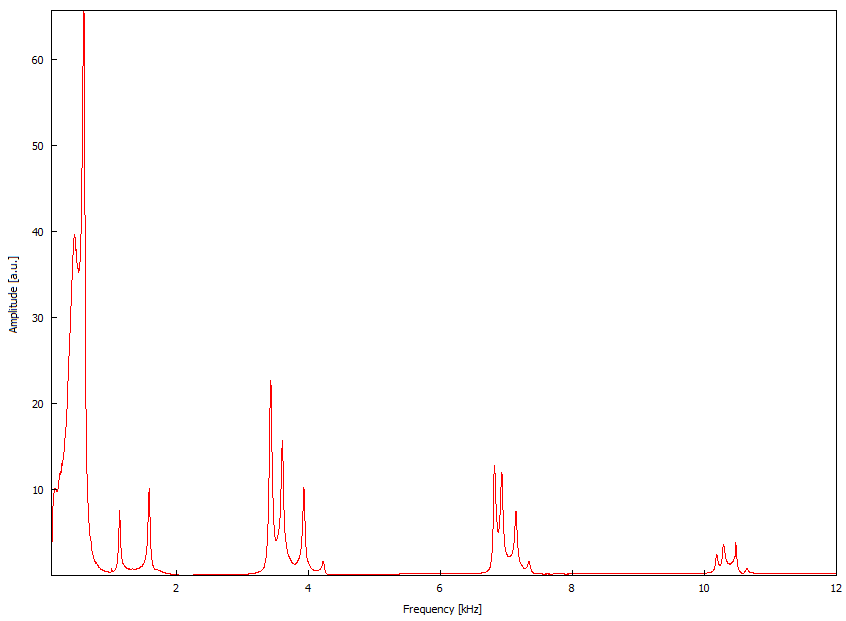
\includegraphics[width=0.45\textwidth]{data/Festkoerper/10mm/Spektrum_4.png}}\hfil
    \subfloat[Frequenzspektrum einer Resonatorkette bestehend aus vier Rohrzylindern der Länge 50mm und eine Blende mit dem Durchmesser von 13mm.]{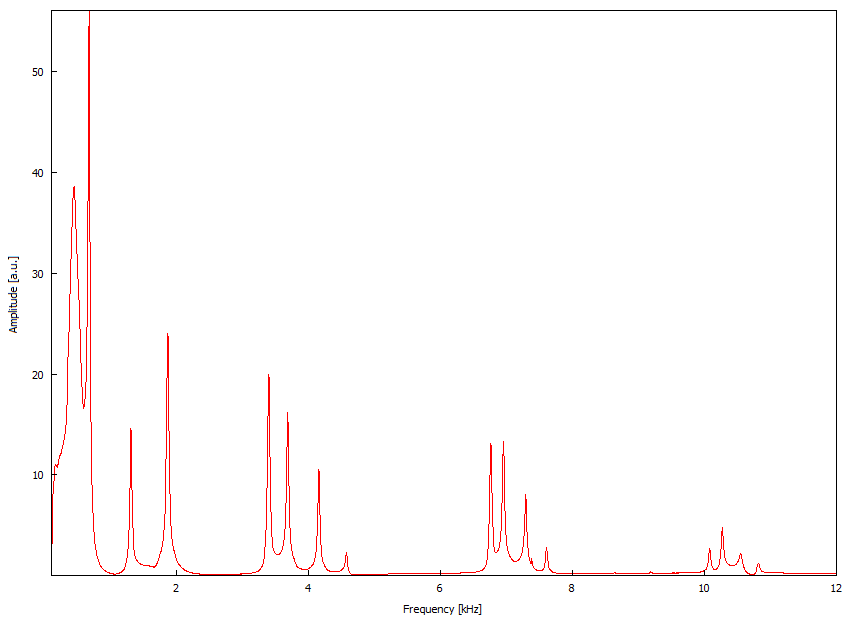
\includegraphics[width=0.45\textwidth]{data/Festkoerper/13mm/Spektrum_4.png}}\hfil 
    \caption{}
    \label{fig:fest_4_blende}
\end{figure}

\begin{figure}[H]
    \centering
    \subfloat[Frequenzspektrum einer Resonatorkette bestehend aus zehn Rohrzylindern der Länge 50mm und eine Blende mit dem Durchmesser von 10mm.]{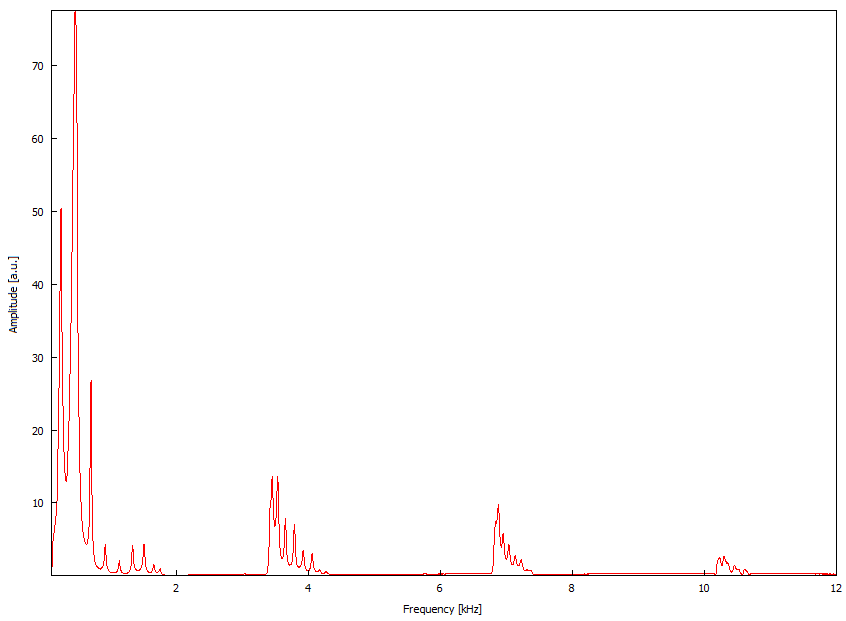
\includegraphics[width=0.45\textwidth]{data/Festkoerper/10mm/Spektrum_10.png}}\hfil
    \subfloat[Frequenzspektrum einer Resonatorkette bestehend aus zehn Rohrzylindern der Länge 50mm und eine Blende mit dem Durchmesser von 13mm.]{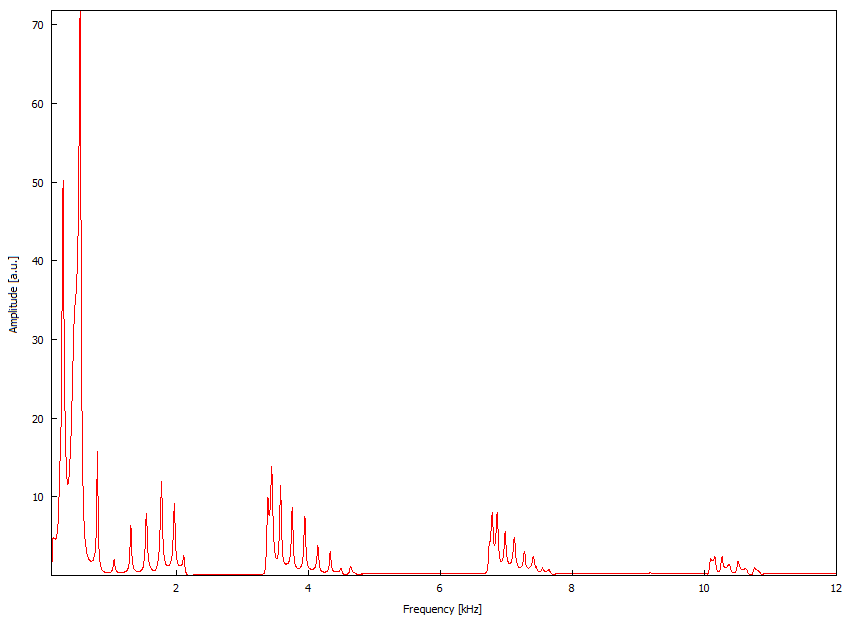
\includegraphics[width=0.45\textwidth]{data/Festkoerper/13mm/Spektrum_10.png}}\hfil 
    \caption{}
    \label{fig:fest_10_blende}
\end{figure}
Es wird deutlich, dass ..............

\subsubsection*{Störstellen im Festkörper}
Durch Verwendung vereinzelt geänderter Zylinderlängen können Störstellen, die im Festkörper Gitterdefekte entsprechen, simuliert werden.
Diese führen zu Abweichungen im Frequenzspektrum, verglichen zum ungestörten Frequenzspektrum.
Konkret lassen sich für die Störzylinder der Größe $?$mm und $?$mm eine neue Resonanz erkennen. Des weiteren resultiert eine
deutlich sichtbare Verringerung der gesamten Druckamplitude im Vergleich zur ungestörten Resonatorkette. 

\begin{figure}[H]
    \centering
    \subfloat[Fehlstelle mit $37,5$mm Zylinder.]{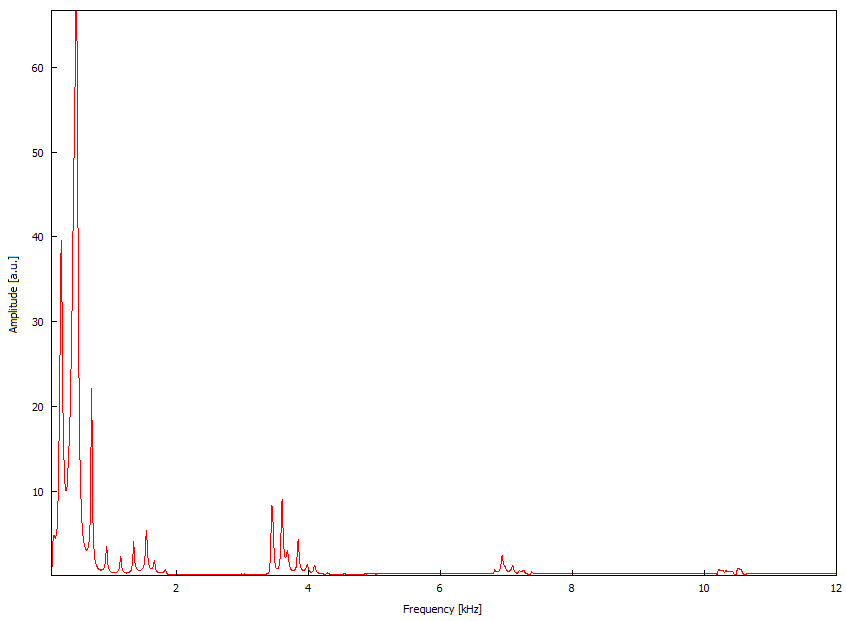
\includegraphics[width=0.45\textwidth]{data/Festkoerper/10mm/Spektrum_dotiert_37_5.png}}\hfil
    \subfloat[Fehlstelle mit $62,5$mm Zylinder.]{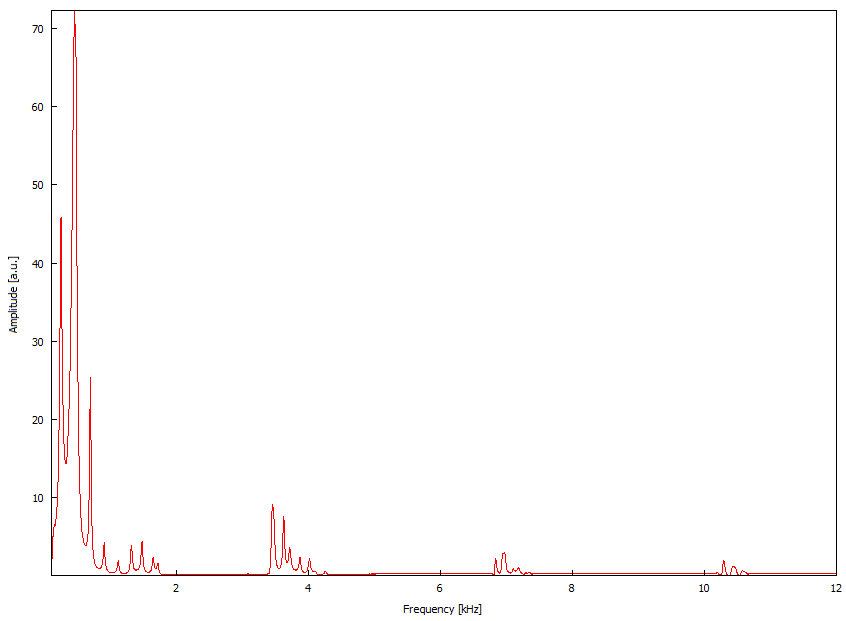
\includegraphics[width=0.45\textwidth]{data/Festkoerper/10mm/Spektrum_dotiert_62_5.png}}\hfil 
    \subfloat[Fehlstelle mit $75$mm Zylinder.]{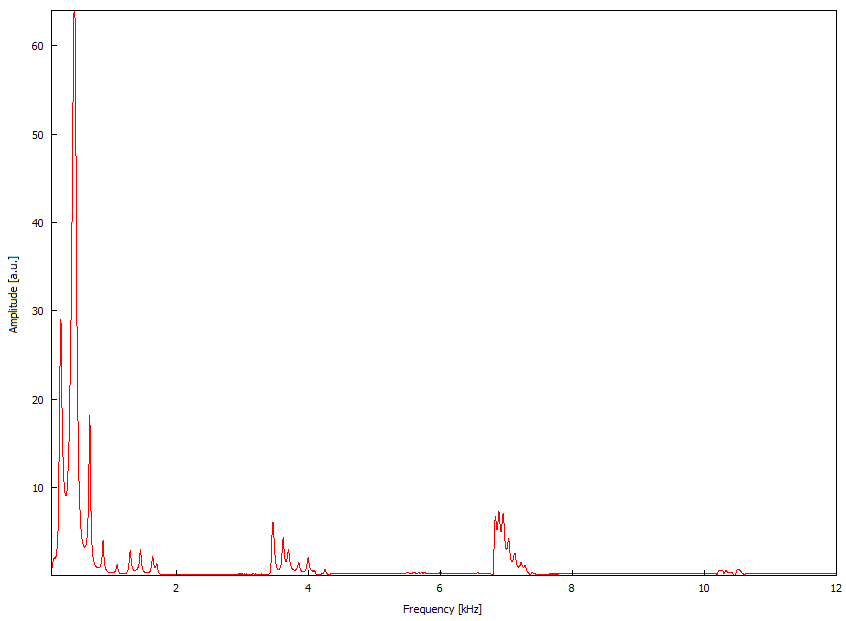
\includegraphics[width=0.45\textwidth]{data/Festkoerper/10mm/Spektrum_dotiert_75.png}} 
    \caption{Frequenzspektren für eine Resonatorkette aus neun Zylindern der Länge $50$mm und einer Störstelle durch einen Zylinder einer anderen Länge. Zwischenstücke bilden $10$mm Blenden.}
    \label{fig:fest_stoer}
\end{figure}

\subsubsection*{Resonatorkette mit wechselnden Zylinderlängen}
Nun wird eine Resonatorkette aus abwechselnden Zylindern mit den Längen $50$mm und $75$mm betrachtet.
Dies entspricht einer zwei-atomigen-Festkörper-Basis. Deutlich werden nun, dass die Resonanzen der einzelnen ein-atomigen Basen in 
die zwei-atomigen-basen übernommen werden.\\
In Abbildung \ref{fig:abwech_zylin} wird nun die wechselnde Resonatorkette mit einer $50$mm und einer $75$mm Resonatorkette verglichen.

\begin{figure}[H]
    \centering
    \subfloat[Frequenzspektrum eines einzelnen Zylinders mit der Länge von $75$mm.]{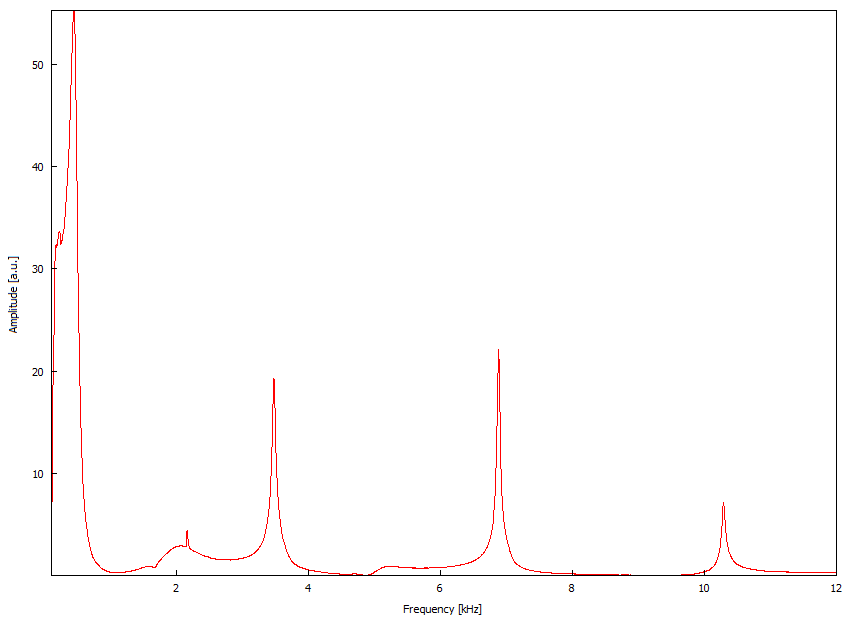
\includegraphics[width=0.5\textwidth]{data/Festkoerper/periodisch/Spektrum_75_einzeln.png}}\hfil
    \subfloat[Frequenzspektrum eines einzelnen Zylinders mit der Länge von $50$mm.]{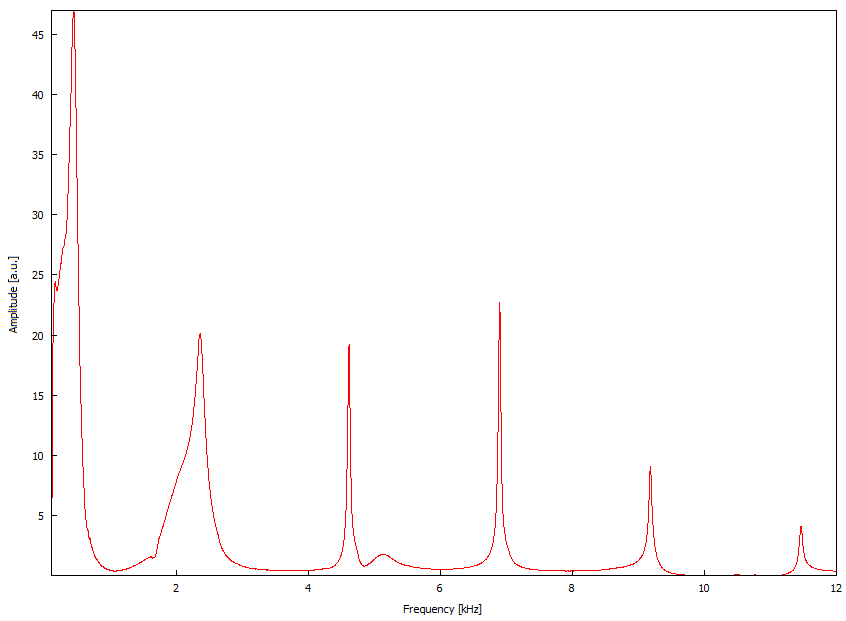
\includegraphics[width=0.5\textwidth]{data/Festkoerper/periodisch/Spektrum_50_einzeln.png}}\hfil 
    \subfloat[Frequenzspektrum einer Resonatorkette mit zehn wechselden Zylindern der Länge $50$mm und $75$mm und Blenden mit einem Durchmesser von $16$mm.]{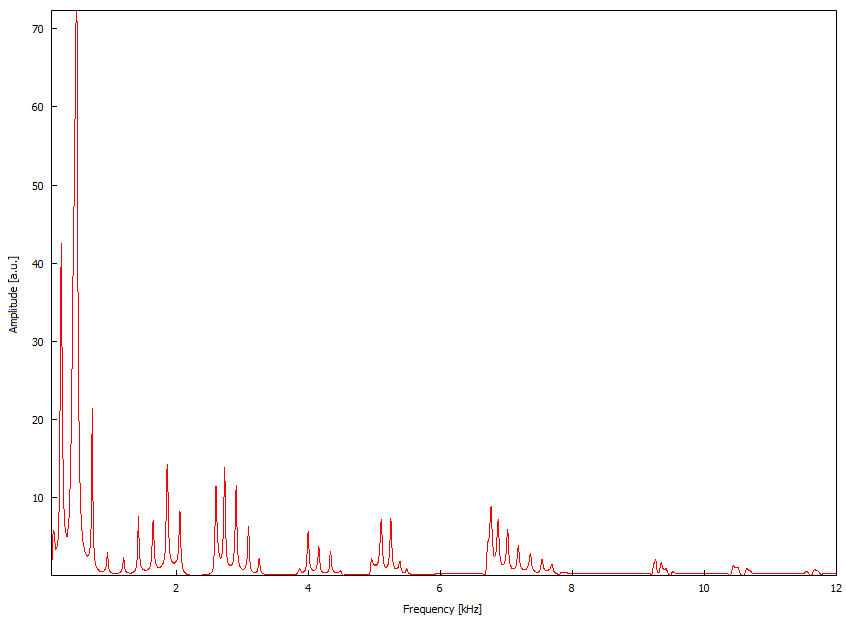
\includegraphics[width=0.8\textwidth]{data/Festkoerper/periodisch/Spektrum_10_16mm_50_75.png}} 
    \caption{}
    \label{fig:abwech_zylin}
\end{figure}

\subsubsection*{Resonatorkette mit wechselndem Blendendurchmesser}
In Abbildung \ref{fig:abwech_blende} ist das Frequenzspektrum einer Resonatorkette aus $?$ Zylindern mit abwechselden Blendendurchmessern
von $13$mm und $16$mm dargestellt. Es zeigt sich eine deutliche Aufspaltung der Maximalbereiche.
Auf einen Festkörper übertragen lässt sich somit sagen, dass das vorliegende Gitter nun eine übergeordnete Periodizität aufweist und diese durch
das verschiedene Potenzial entsteht.

\begin{figure}
    \center
    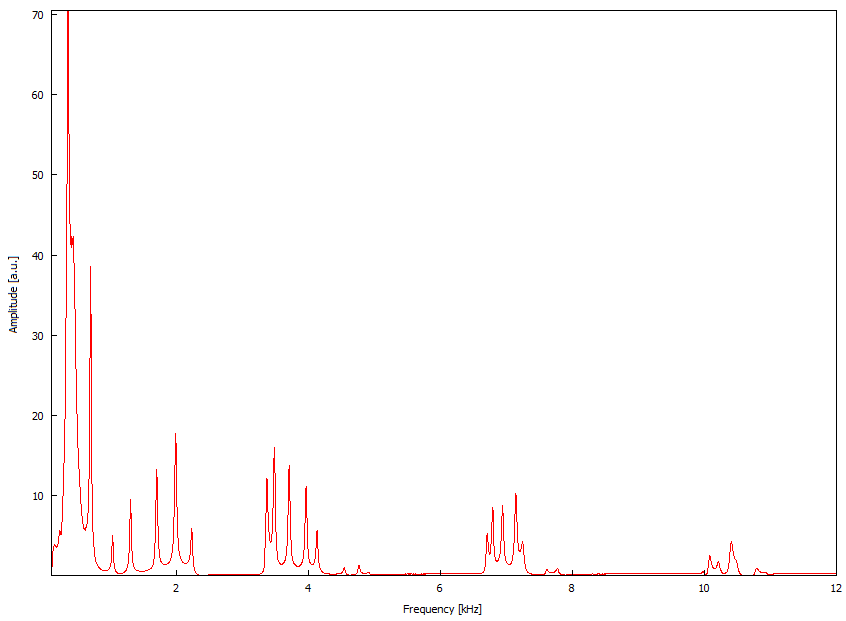
\includegraphics[width=0.8\textwidth]{data/Festkoerper/periodisch/Spektrum_8_13mm_16mm_50.png}
    \caption{Frequenzspektrum einer Resonatorkette aus acht $50$mm langen Zylindern, welche abwechselnd durch $13$mm und $16$mm-Blenden getrennt sind.}
    \label{fig:abwech_blende}
\end{figure}
